\documentclass[12pt]{article}
%%% DOCUMENT FORMATTING %%%
\usepackage[margin=1in]{geometry}
\usepackage{enumitem}
\setlength{\parindent}{0pt}
\newcommand{\disp}{\displaystyle}

%%% HEADER %%%
\usepackage{fancyhdr}
\pagestyle{fancy}
\fancyhf{}
\lhead{MATH 1080}
\rhead{Vagnozzi}
\cfoot{\thepage}

%%% MATH NOTATION & SYMBOLS %%%
\usepackage{amssymb}
\usepackage{amsmath}
\newcommand{\R}{\mathbb{R}}
\newcommand{\N}{\mathbb{N}}
\newcommand{\Z}{\mathbb{Z}}
\newcommand{\lp}{\left(}
\newcommand{\rp}{\right)}
\newcommand{\ls}{\left[}
\newcommand{\rs}{\right]}
\newcommand{\lb}{\left\{}
\newcommand{\rb}{\right\}}
\newcommand{\arccot}{\text{arccot}}
\newcommand{\arccsc}{\text{arccsc}}
\newcommand{\arcsec}{\text{arcsec}} 

%%% TABLES %%%
\usepackage{colortbl}

%%% GRAPHS %%%
\usepackage{tikz}
\usepackage{pgfplots}
\pgfplotsset{compat=1.15}
\usepgfplotslibrary{fillbetween}
\usetikzlibrary{angles,quotes}

%%% ENVIRONMENTS %%%
\newcommand{\Example}{\paragraph{\Writinghand \hspace{0.1mm} Example.}}
\newcommand{\ExampleCont}{\paragraph{\Writinghand \hspace{0.1mm} Example (continued).}}
\newcommand{\boxenv}[2]{
	\fbox{
	\begin{minipage}{0.97\textwidth}
	\vspace{2mm}	
	\paragraph{#1} #2
	\vspace{2mm}
	\end{minipage}
	}}

%%% FUN THINGS %%%
\newcommand*\tc[1]{\tikz[baseline=(char.base)]{
            \node[shape=circle,draw,inner sep=2pt] (char) {#1};}}
\usepackage{marvosym}

%%% MISC %%%
\usepackage{hyperref}


\setcounter{page}{81}

\begin{document}
\section*{8.9: Improper Integrals}

\boxenv{Learning Objectives.}{Upon successful completion of Section 8.9, you will be able to\dots
		
	\begin{itemize}[leftmargin=6mm]
		\item Answer conceptual questions involving improper integrals.
		\item Evaluate improper integrals with an infinite limit of integration.
		\item Evaluate improper integrals with unbounded integrands.
		\item Find areas and volumes using improper integrals.
		\item Use the comparison test to determine whether an integral converges or diverges.
	\end{itemize}
	\vspace{-4mm}
}

\vspace{5mm}

\subsection*{Motivating Application}

The energy required to launch a rocket from the surface of Earth ($R=6370$ km from the center of Earth) to an altitude $H$ is given by an integral of the form 

$$\int_R^{R+H}\frac{k}{x^2}\,dx,$$

\vspace{2mm}

where $k$ is a constant that includes the mass of the rocket, the mass of Earth, and the gravitational constant. Suppose we want to launch the rocket to an arbitrarily large altitude~$H$ so that it escapes Earth's gravitational field. Then the energy required is

$$\int_R^\infty\frac{k}{x^2}\,dx.$$

\vspace{4mm}

How could we evaluate this integral? Let's think back to one of our fundamental theorems.\\

\boxenv{Second Fundamental Theorem of Calculus.}{Let $f$ be continuous on $[a,b]$ and \\ suppose that $F$ is an antiderivative for $f$ on the same interval. Then
$$\int_a^b f(x)\,dx=\int_a^b F'(x)\,dx=F(b)-F(a).$$
\vspace{-3mm}
}

\vspace{3mm}

\newpage

\Example Consider the following two integrals. Does the Second Fundamental Theorem of Calculus apply? Why or why not?\\

\begin{multicols}{2}

\begin{itemize}
	\item[\tc{1}] $\disp\int_1^\infty\frac{1}{x}\,dx$
	
	\vfill
	
	\item[\tc{2}] $\disp\int_0^1\frac{1}{x}\,dx$
	
	\vfill
\end{itemize}
\begin{flushright}

\begin{tikzpicture}[scale=.8]
	\begin{axis}[grid=none,
    	axis x line=middle,
        xmax=5.2, xmin=-5.2,
        axis y line=center,
        ymax=5.2, ymin=-5.2,
        axis line style=<->,
%		xlabel=$x$,ylabel=$y$,
		xticklabels={},
		yticklabels={},
		xtick={-5,-4,...,5},
		ytick={-5,-4,...,5},
		axis on top                    	
		]
    \addplot[<->,name path=f,smooth,domain=0.2:5,color=blue,samples=100,very thick] {1/x};
    \addplot[<->,name path=f,smooth,domain=-5:-0.2,color=blue,samples=100,very thick] {1/x};
    \end{axis}
\end{tikzpicture}

\vspace{5mm}

\begin{tikzpicture}[scale=.8]
	\begin{axis}[grid=none,
    	axis x line=middle,
        xmax=5.2, xmin=-5.2,
        axis y line=center,
        ymax=5.2, ymin=-5.2,
        axis line style=<->,
%		xlabel=$x$,ylabel=$y$,
		xticklabels={},
		yticklabels={},
		xtick={-5,-4,...,5},
		ytick={-5,-4,...,5},
		axis on top                    	
		]
    \addplot[<->,name path=f,smooth,domain=0.2:5,color=blue,samples=100,very thick] {1/x};
    \addplot[<->,name path=f,smooth,domain=-5:-0.2,color=blue,samples=100,very thick] {1/x};
    \end{axis}
\end{tikzpicture}
\end{flushright}

\end{multicols}

\subsection*{Improper Integrals of Type~1}

\begin{itemize}
\item[(a)] If $f(x)$ is continuous on $[a,\infty)$, then\\

$\disp\int_a^\infty f(x)\,dx=$

\vfill

\item[(b)] If $f(x)$ is continuous on $(-\infty,b]$, then\\

$\disp\int_{-\infty}^b f(x)\,dx=$

\vfill

\end{itemize}

\noindent We say that an integral \textbf{converges} if the limit exists. Otherwise, we say it \textbf{diverges}.

\newpage

\begin{itemize}

\item[(c)] If $f(x)$ is continuous on $(-\infty,\infty)$, then\\

$\disp\int_{-\infty}^\infty f(x)\,dx=$

\vspace{40mm}

\end{itemize}

\Example Find the area under the curve $y=\disp\frac{1}{x}$ for $x\geq 1$.

\begin{flushright}
\begin{tikzpicture}[scale=1]
	\begin{axis}[grid=none,
    	axis x line=middle,
        xmax=4.2, xmin=-4.2,
        axis y line=center,
        ymax=4.2, ymin=-4.2,
        axis line style=<->,
%		xlabel=$x$,ylabel=$y$,
		xticklabels={},
		yticklabels={},
		xtick=\empty,
		ytick=\empty,
		axis on top                    	
		]
    \addplot[<->,name path=f,smooth,domain=0.25:4,color=blue,samples=100,very thick] {1/x};
    \addplot[<->,name path=f,smooth,domain=-4:-0.25,color=blue,samples=100,very thick] {1/x};
    \end{axis}
\end{tikzpicture}
\end{flushright}


\newpage

\Example Find the volume of the solid generated when $y=\disp\frac{1}{x}$ for $x\geq 1$ is rotated about the $x$-axis.

\begin{flushright}
\begin{tikzpicture}[scale=1]
	\begin{axis}[grid=none,
    	axis x line=middle,
        xmax=4.2, xmin=-4.2,
        axis y line=center,
        ymax=4.2, ymin=-4.2,
        axis line style=<->,
%		xlabel=$x$,ylabel=$y$,
		xticklabels={},
		yticklabels={},
		xtick=\empty,
		ytick=\empty,
		axis on top                    	
		]
    \addplot[<->,name path=f,smooth,domain=0.25:4,color=blue,samples=100,very thick] {1/x};
    \addplot[<->,name path=f,smooth,domain=-4:-0.25,color=blue,samples=100,very thick] {1/x};
    \end{axis}
\end{tikzpicture}
\end{flushright}

\vfill

\textbf{Fact:} $\disp\int_1^\infty\frac{1}{x^p}\,dx$ \textbf{converges} for \underline{\hspace{30mm}} and \textbf{diverges} for \underline{\hspace{30mm}}.

\newpage

\Example Evaluate $\disp\int_0^\infty \frac{x}{\sqrt{x^4+1}}\,dx$.

\newpage

\subsection*{Improper Integrals with an Unbounded Integrand (Type~2)}

\begin{itemize}

\item[(a)] If $f(x)$ is continuous on $(a,b]$ with $\disp\lim_{x\to a^+}f(x)=\pm\infty$, then\\

$\disp\int_a^bf(x)\,dx=$

\vspace{40mm}

\item[(b)] If $f(x)$ is continuous on $[a,b)$ with $\disp\lim_{x\to b^-}f(x)=\pm\infty$, then\\

$\disp\int_a^b f(x)\,dx=$

\vspace{40mm}

\item[(c)] If $f(x)$ is continuous on $[a,b]$ except at the interior point $p$ where $f$ is unbounded, then\\

$\disp\int_a^b f(x)\,dx=$

\vspace{40mm}
\end{itemize}


\newpage

\Example Evaluate $\disp\int_{-1}^1\frac{1}{x}\,dx$.

\begin{flushright}

\vspace{-15mm}
\begin{tikzpicture}[scale=1]
	\begin{axis}[grid=none,
    	axis x line=middle,
        xmax=4.2, xmin=-4.2,
        axis y line=center,
        ymax=4.2, ymin=-4.2,
        axis line style=<->,
%		xlabel=$x$,ylabel=$y$,
		xticklabels={},
		yticklabels={},
		xtick=\empty,
		ytick=\empty,
		axis on top                    	
		]
    \addplot[<->,name path=f,smooth,domain=0.25:4,color=blue,samples=100,very thick] {1/x};
    \addplot[<->,name path=f,smooth,domain=-4:-0.25,color=blue,samples=100,very thick] {1/x};
    \end{axis}
\end{tikzpicture}
\end{flushright}

\newpage

\Example Evaluate $\disp\int_0^8\frac{1}{\sqrt[3]{x}}\,dx$.

\newpage

\Example Evaluate $\disp\int_0^{\pi/2}\tan\theta\,d\theta$.

\begin{flushright}

\vspace{-15mm}
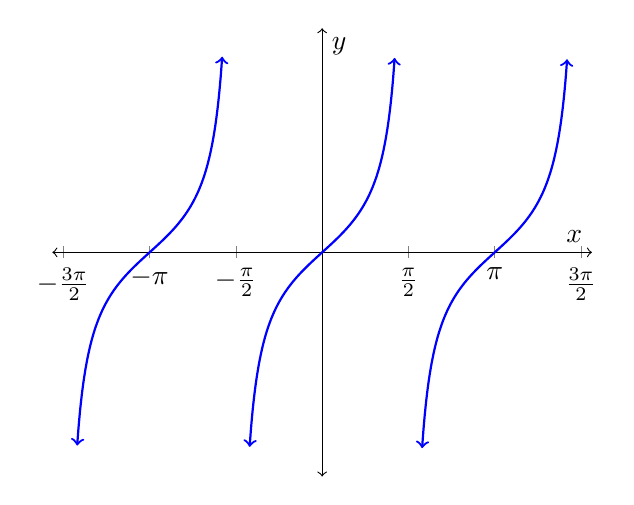
\begin{tikzpicture}
                \begin{axis}[
                	axis x line=middle,
                	xmax=3*pi/2+.2, xmin=-3*pi/2-.2,
                	axis y line=center,
                	ymax=4.5, ymin=-4.5,
                	axis line style={<->},
                	xlabel=$x$,ylabel=$y$,
                	ytick=\empty,
                	xtick={-3*pi/2,-pi,-pi/2,0,pi/2,pi,3*pi/2},
                	xticklabels={$-\frac{3\pi}{2}$,$-\pi$,$-\frac{\pi}{2}$,0,$\frac{\pi}{2}$,$\pi$,$\frac{3\pi}{2}$}
                    ]
%                    \addplot[name path=f,smooth,domain=-2*pi-.4:-4.96,color=blue,samples=100,<->,thick] {tan(deg(x))}; 
                	\addplot[name path=f,smooth,domain=-4.46:-1.82,color=blue,samples=100,<->,thick] {tan(deg(x))};      
                	\addplot[name path=f,smooth,domain=-1.32:1.32,color=blue,samples=100,<->,thick] {tan(deg(x))};      
                	\addplot[name path=f,smooth,domain=1.82:4.46,color=blue,samples=100,<->,thick] {tan(deg(x))};      
%                	\addplot[name path=f,smooth,domain=4.95:2*pi+.4,color=blue,samples=100,<->,thick] {tan(deg(x))};      
                     \end{axis}
            \end{tikzpicture}
\end{flushright}

\newpage

\Example Evaluate $\disp\int_0^1\ln x\,dx$.

\newpage

\subsection*{Comparison Theorem for Improper Integrals}

\boxenv{Comparison Theorem.}{Suppose $f$, $g$ are continuous functions with $f(x)\geq g(x)\geq 0$, for $x \geq a$.\\

If $\disp\int_a^\infty f(x)\,dx$ converges, then 

\vspace{6mm}

If $\disp\int_a^\infty g(x)\,dx$ diverges, then 

}

\vspace{5mm}

\textbf{Caution:} We have to be careful with what we conclude using the Comparison Theorem.

\vspace{5mm}

If $\disp\int_a^\infty f(x)\,dx$ diverges, then

\vspace{23mm}

If $\disp\int_a^\infty g(x)\,dx$ converges, then

\vspace{23mm}

\Example Determine whether $\disp\int_1^\infty e^{-x^2}\,dx$ converges or diverges.

\newpage

\boxenv{Recall:}{$\disp\int_1^\infty\frac{1}{x^p}\,dx$ \textbf{converges} for $p\geq 1$ and \textbf{diverges} for $p\leq 1$.}


\Example Determine whether $\disp\int_1^\infty\frac{2+e^{-x}}{x}\,dx$ converges or diverges.

\vfill

\Example Determine whether $\disp\int_1^\infty\frac{x}{x^3+1}\,dx$ converges or diverges.

\vfill
\end{document}